%% LyX 1.3 created this file.  For more info, see http://www.lyx.org/.
%% Do not edit unless you really know what you are doing.
\documentclass[english, 12pt]{article}
\usepackage{times}
%\usepackage{algorithm2e}
\usepackage{url}
\usepackage{bbm}
\usepackage[T1]{fontenc}
\usepackage[latin1]{inputenc}
\usepackage{geometry}
\geometry{verbose,letterpaper,tmargin=2cm,bmargin=2cm,lmargin=1.5cm,rmargin=1.5cm}
\usepackage{rotating}
\usepackage{color}
\usepackage{graphicx}
\usepackage{amsmath, amsthm, amssymb}
\usepackage{setspace}
\usepackage{lineno}
\usepackage{hyperref}
\usepackage{bbm}
\usepackage{makecell}
\usepackage{placeins}
\usepackage{subcaption}

%\renewcommand{\arraystretch}{1.8}

%\linenumbers
%\doublespacing
\onehalfspacing
%\usepackage[authoryear]{natbib}
\usepackage{natbib} \bibpunct{(}{)}{;}{author-year}{}{,}

%Pour les rajouts
\usepackage{color}
\definecolor{trustcolor}{rgb}{0,0,1}

\usepackage{dsfont}
\usepackage[warn]{textcomp}
\usepackage{adjustbox}
\usepackage{multirow}
\usepackage{subcaption}
\usepackage{graphicx}
\graphicspath{{../figures/}}
\DeclareMathOperator*{\argmin}{\arg\!\min}

\let\tabbeg\tabular
\let\tabend\endtabular
\renewenvironment{tabular}{\begin{adjustbox}{max width=0.95\textwidth}\tabbeg}{\tabend\end{adjustbox}}

\makeatletter

%%%%%%%%%%%%%%%%%%%%%%%%%%%%%% LyX specific LaTeX commands.
%% Bold symbol macro for standard LaTeX users
%\newcommand{\boldsymbol}[1]{\mbox{\boldmath $#1$}}

%% Because html converters don't know tabularnewline
\providecommand{\tabularnewline}{\\}
\renewcommand*{\arraystretch}{1.2}

\usepackage{babel}
\makeatother


\begin{document}

\renewcommand{\thefigure}{S\arabic{figure}}
\setcounter{figure}{0}
\renewcommand{\thetable}{S\arabic{table}}
\setcounter{table}{0}
\renewcommand{\theequation}{S\arabic{equation}}
\setcounter{equation}{0}

\section*{Supplementary Tables and Figures}

%%%%%%%%%%%%%%%%%%%%%%%%%%%%%%%%%%%%%%%%%%%%%%%%%%%%%%%%%%%%%%%%%%%%%%%%%%%%%%%%

\begin{figure}[htbp]
	\centerline{\includegraphics[width=0.9\textwidth]{ratio-dist}}
	\caption{Relative predictive performance with UK compared to the PC distance with UK between centers of ancestry groups \cite[]{prive2020ancestry}. Relative performance values are the ones reported in Figure 1 of the main text.}
	\label{fig:ratio-dist}
\end{figure}

\begin{figure}[h]
	\centering
	\includegraphics[width=0.9\textwidth]{lasso-ancestry-geno}
	\caption{}
	\label{fig:lasso-ancestry-geno}
\end{figure}

\begin{figure}[h]
\centering
\includegraphics[width=0.9\textwidth]{ldpred2-ancestry}
\caption{}
\label{fig:ldpred2-ancestry}
\end{figure}

%%%%%%%%%%%%%%%%%%%%%%%%%%%%%%%%%%%%%%%%%%%%%%%%%%%%%%%%%%%%%%%%%%%%%%%%%%%%%%%%

\begin{figure}[h]
	\centering
	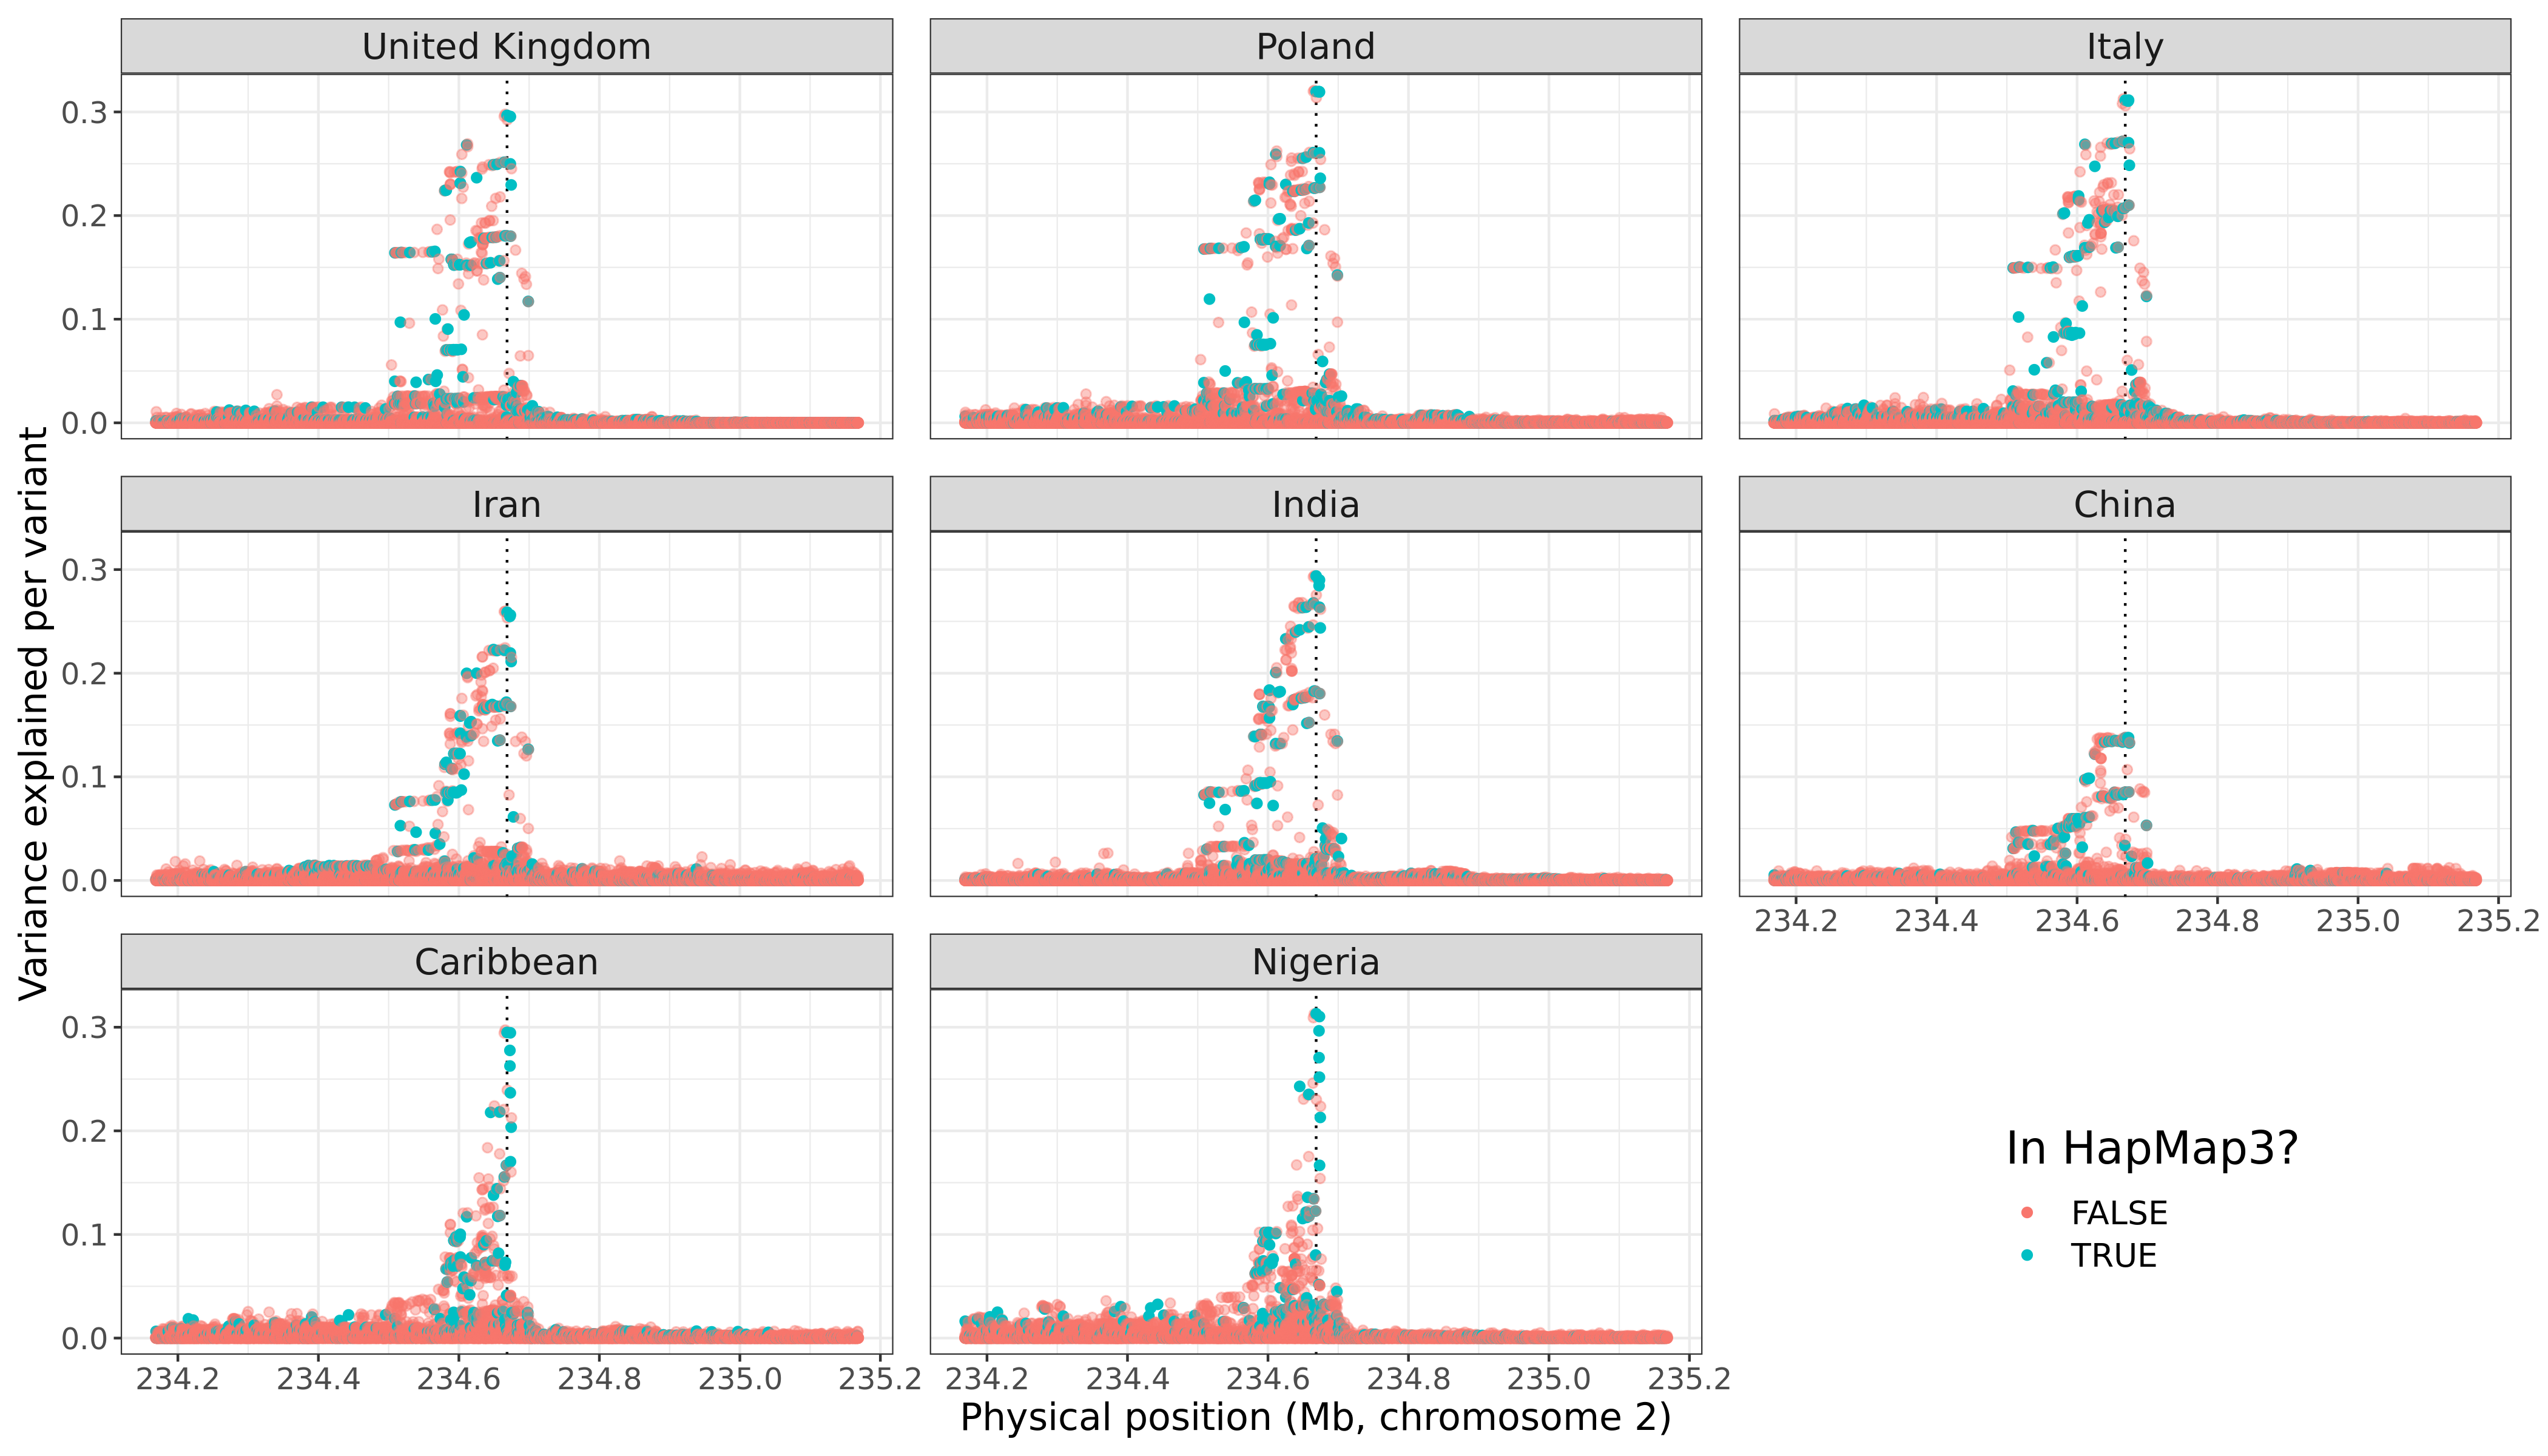
\includegraphics[width=0.9\textwidth]{zoom_log_bilirubin}
	\caption{}
	\label{fig:zoom-bilirubin}
\end{figure}

\begin{figure}[h]
	\centering
	\includegraphics[width=0.9\textwidth]{top3_log_bilirubin}
	\caption{}
	\label{fig:top3-bilirubin}
\end{figure}

\begin{figure}[h]
	\centering
	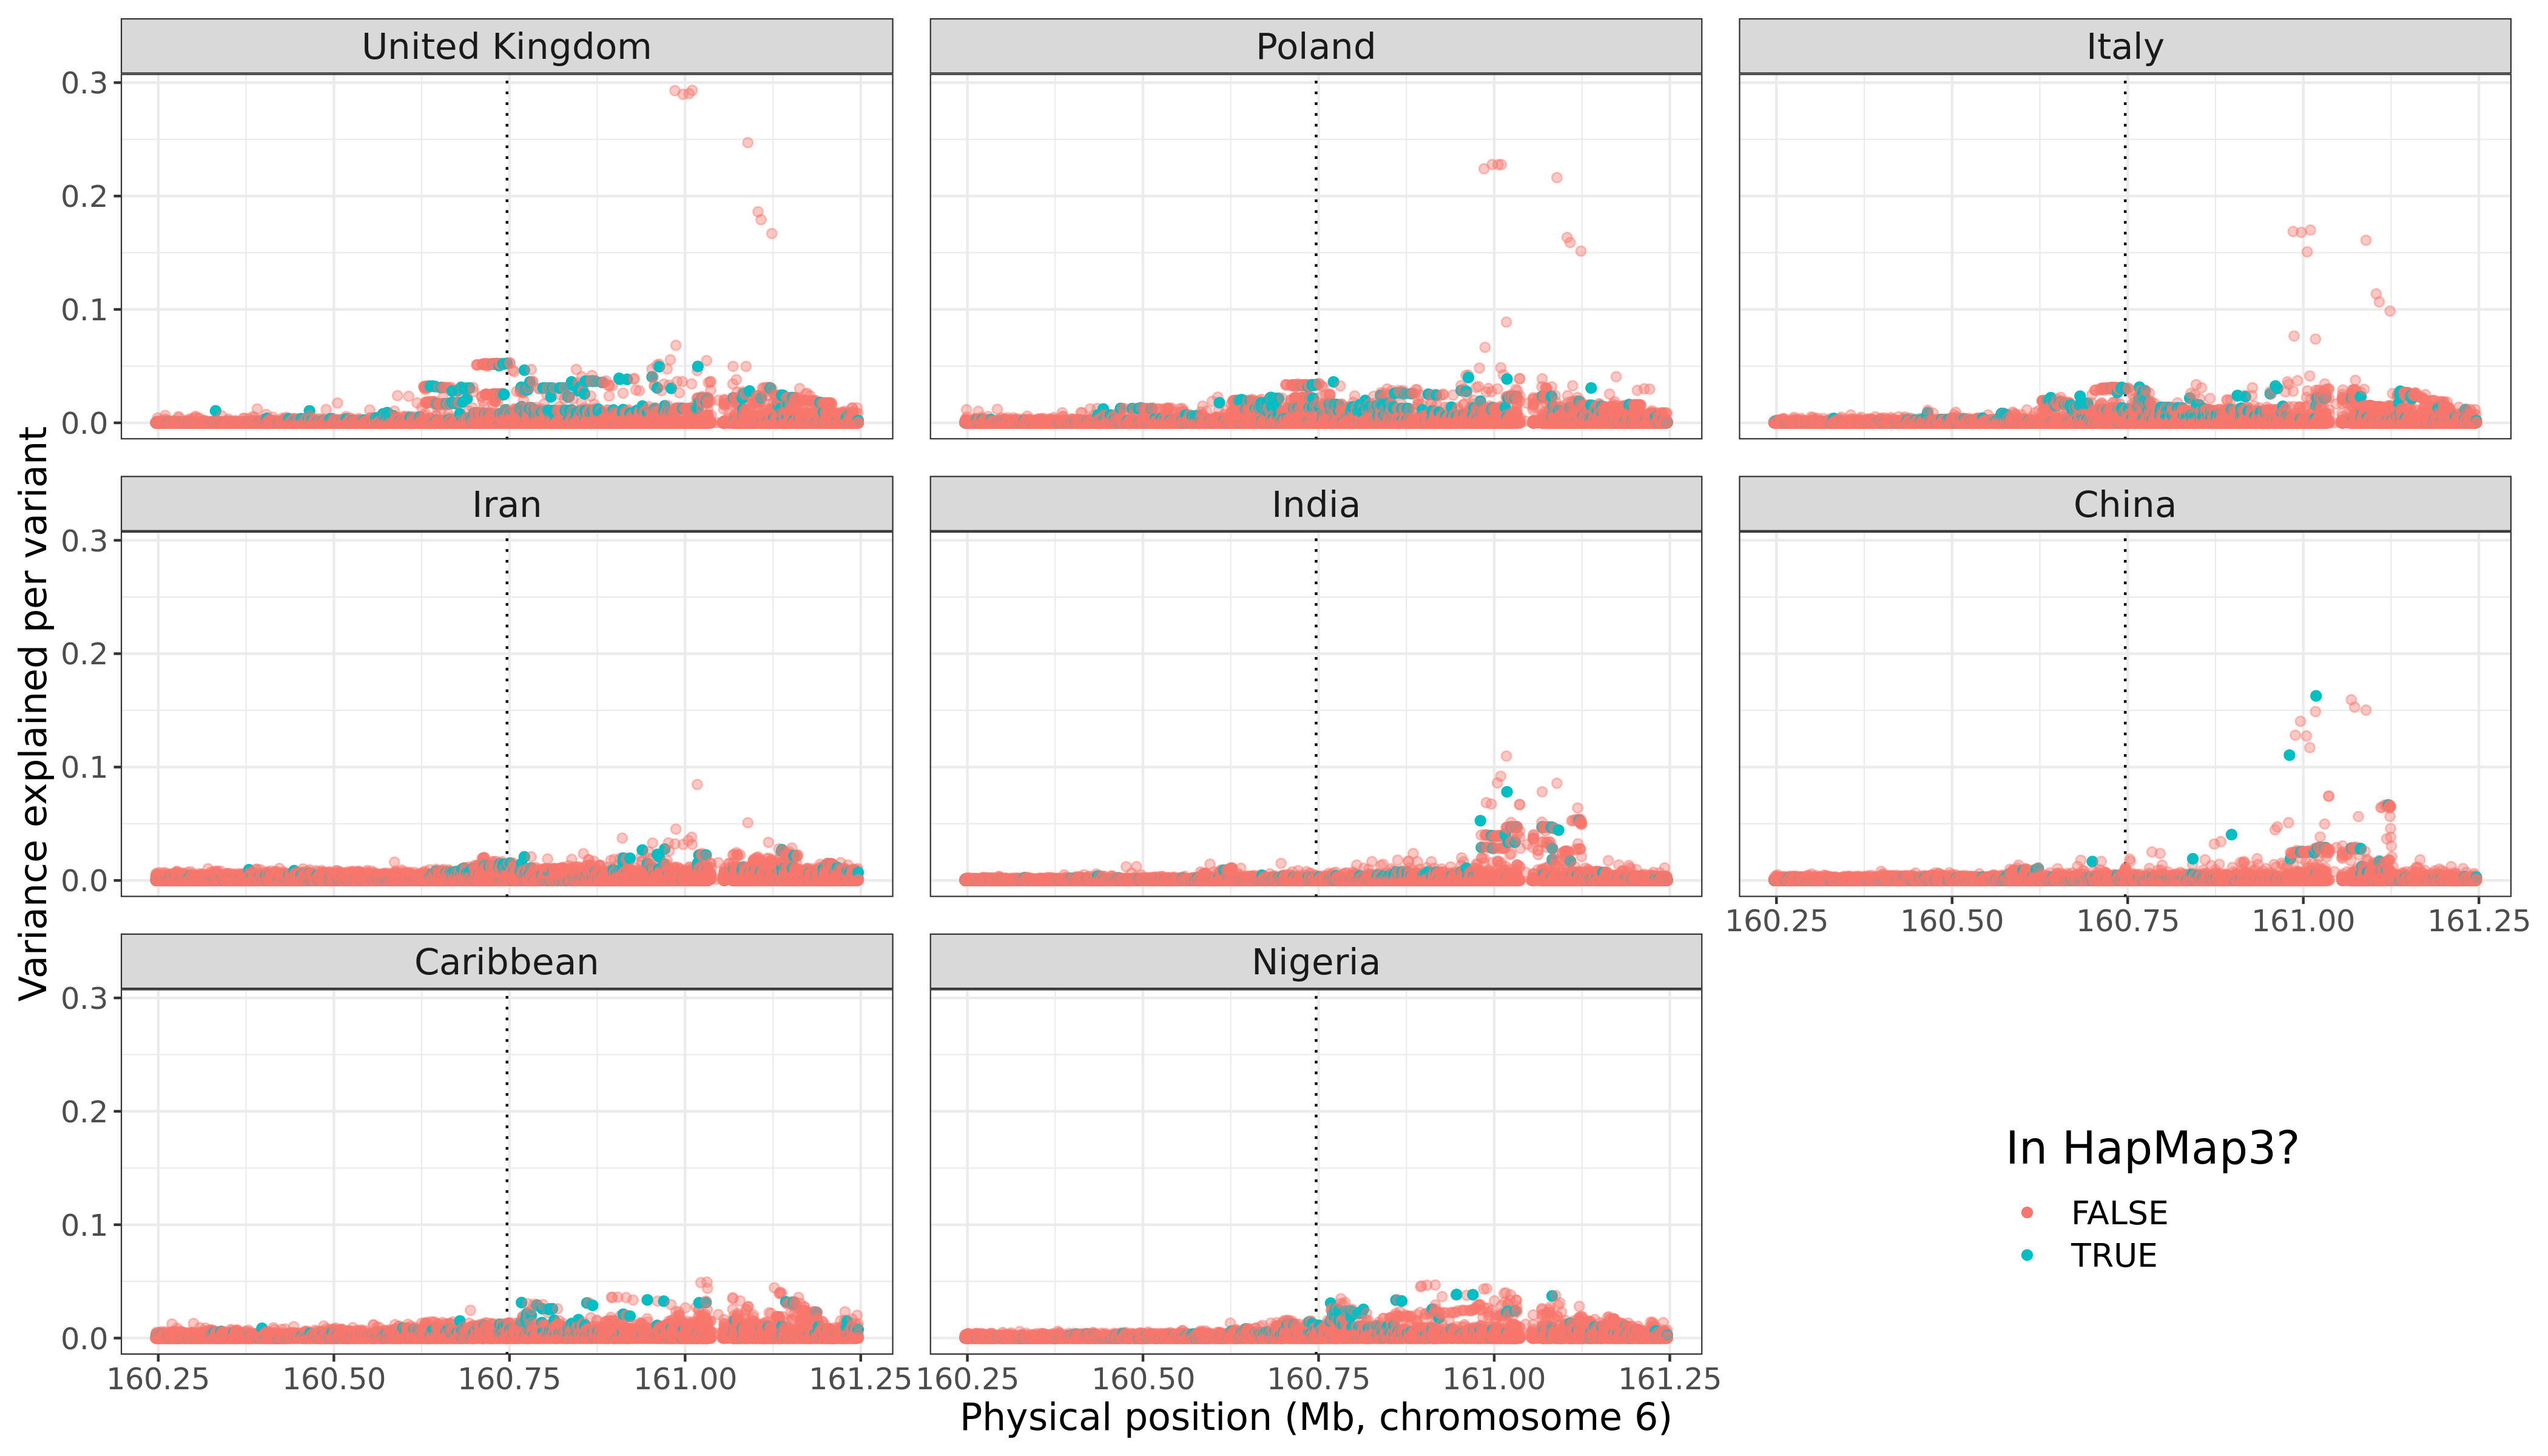
\includegraphics[width=0.9\textwidth]{zoom_log_lipoA}
	\caption{}
	\label{fig:zoom-lipoA}
\end{figure}

\begin{figure}[h]
	\centering
	\includegraphics[width=0.9\textwidth]{top3_log_lipoA}
	\caption{}
	\label{fig:top3-lipoA}
\end{figure}

\begin{figure}[h]
	\centering
	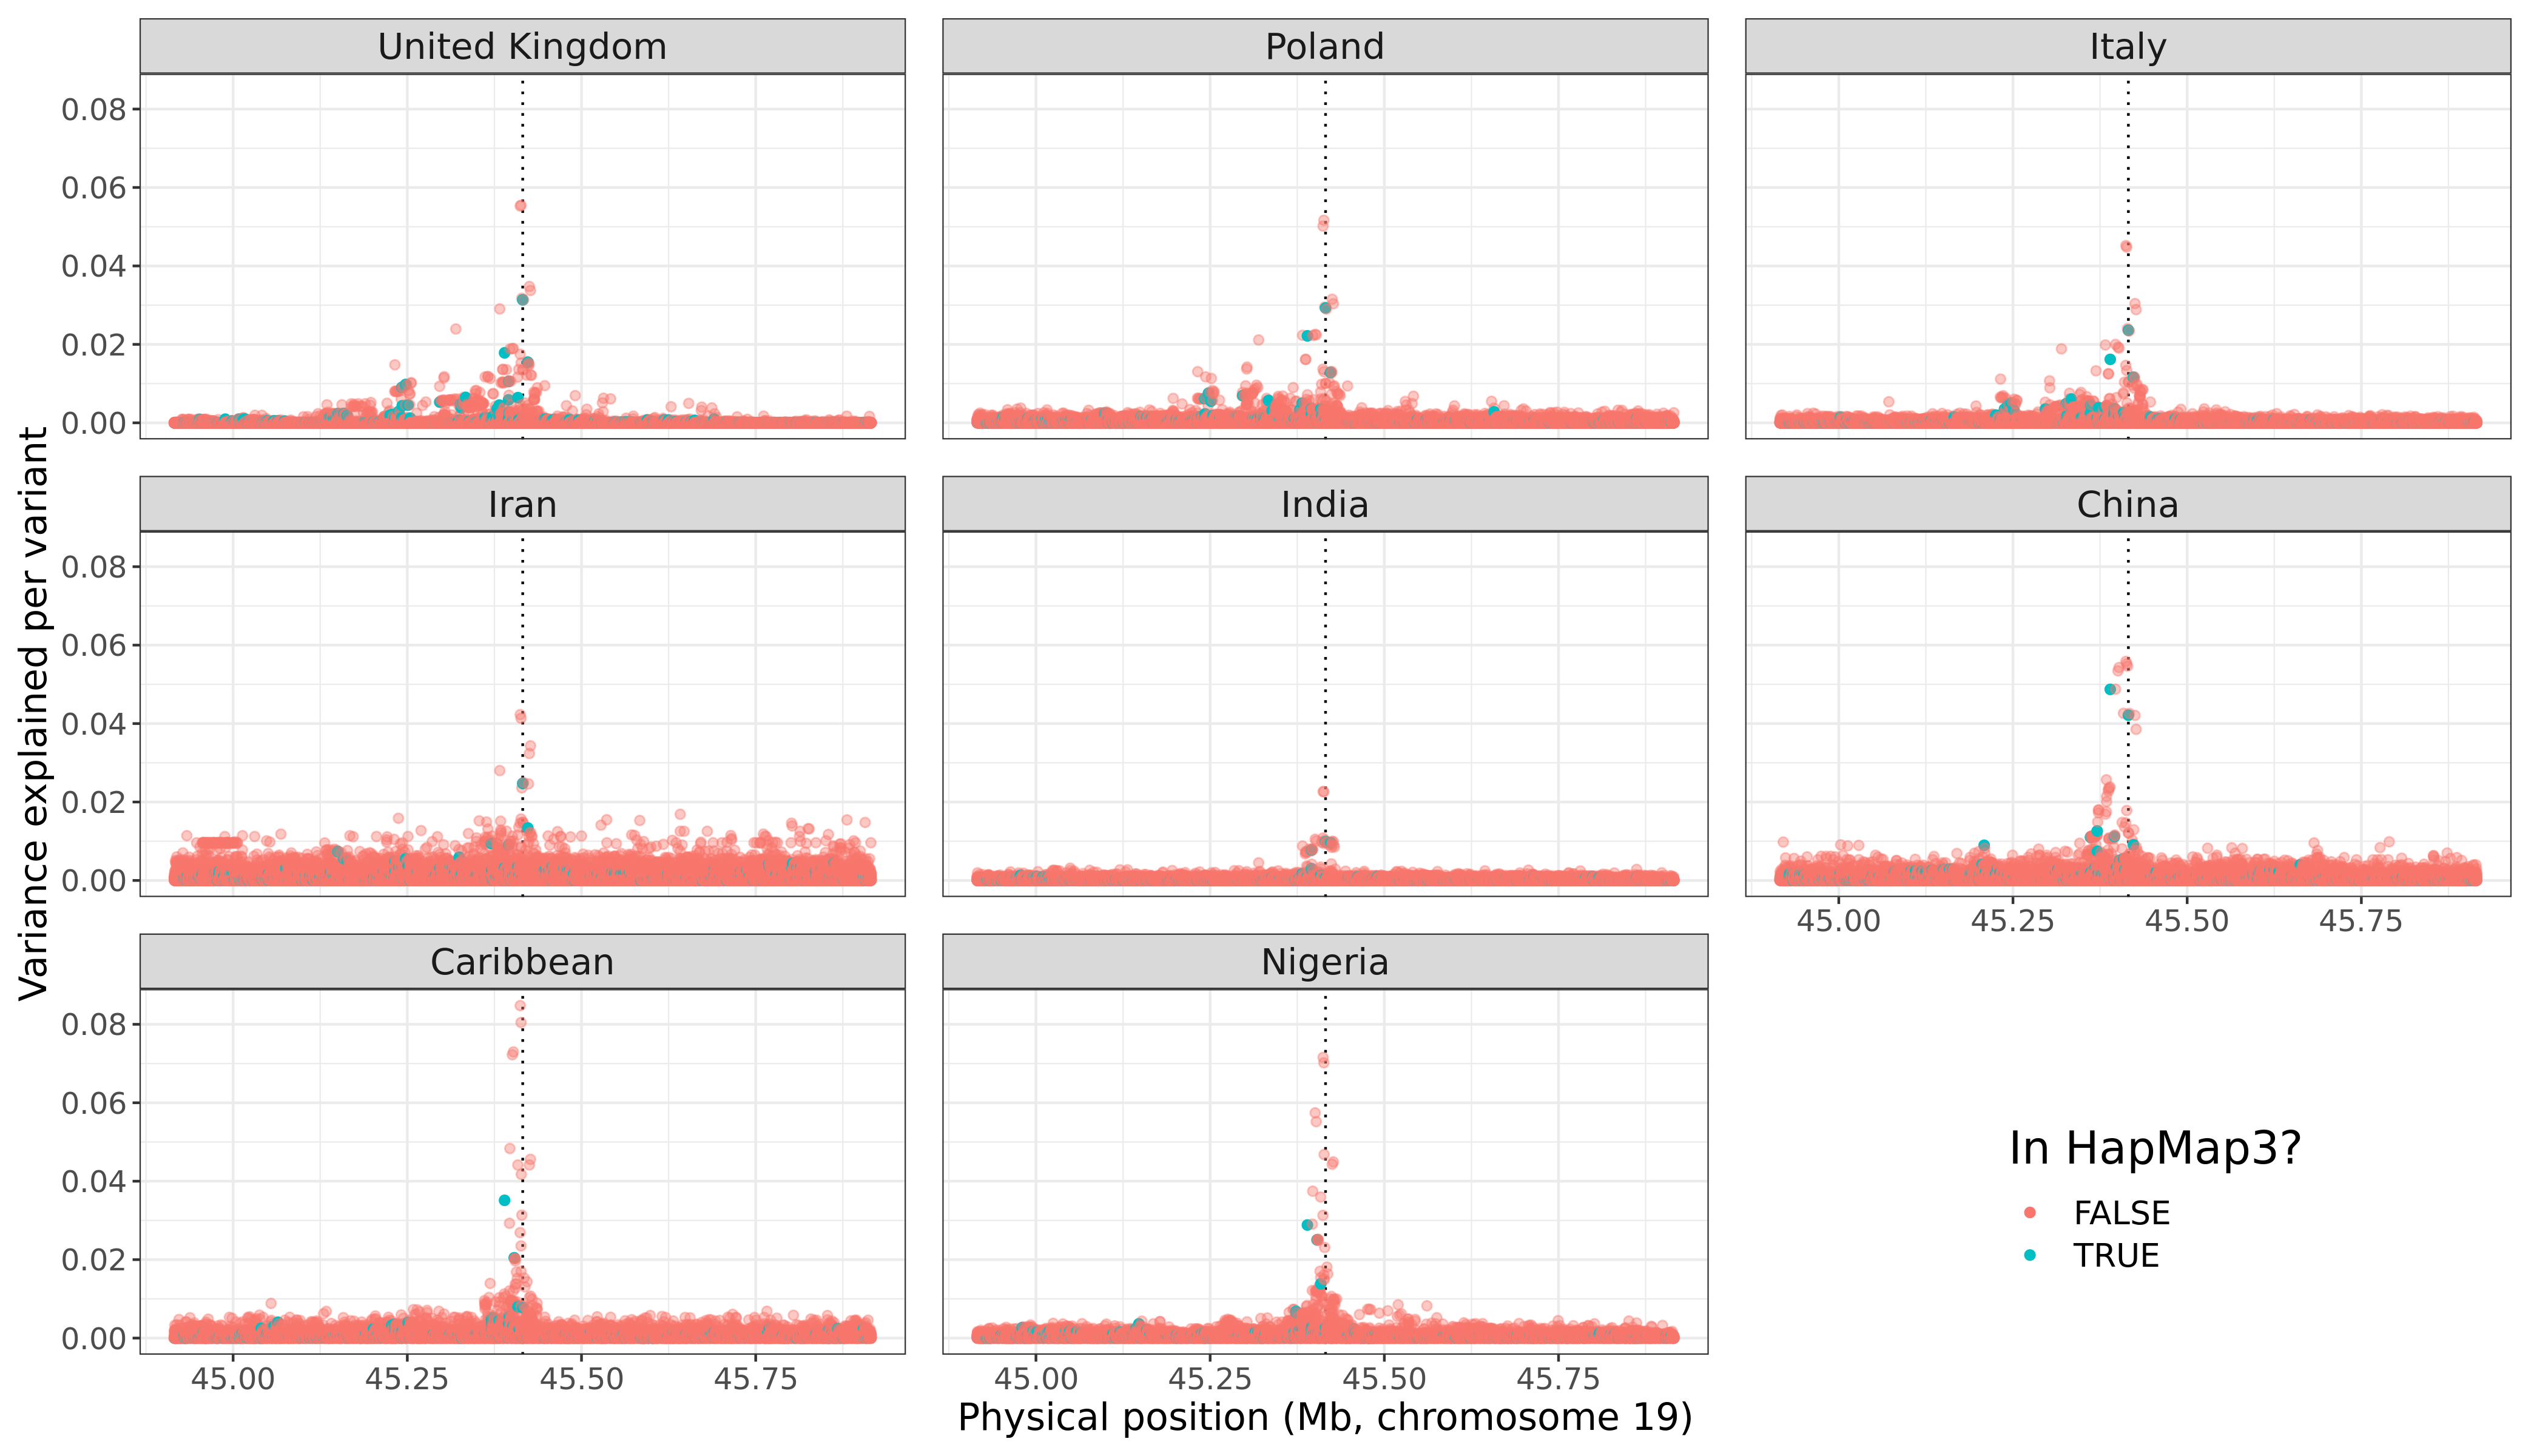
\includegraphics[width=0.9\textwidth]{zoom_apoB}
	\caption{}
	\label{fig:zoom-apoB}
\end{figure}

\begin{figure}[h]
	\centering
	\includegraphics[width=0.9\textwidth]{top3_apoB}
	\caption{}
	\label{fig:top3-apoB}
\end{figure}

%%%%%%%%%%%%%%%%%%%%%%%%%%%%%%%%%%%%%%%%%%%%%%%%%%%%%%%%%%%%%%%%%%%%%%%%%%%%%%%%

\begin{figure}[h]
	\centering
	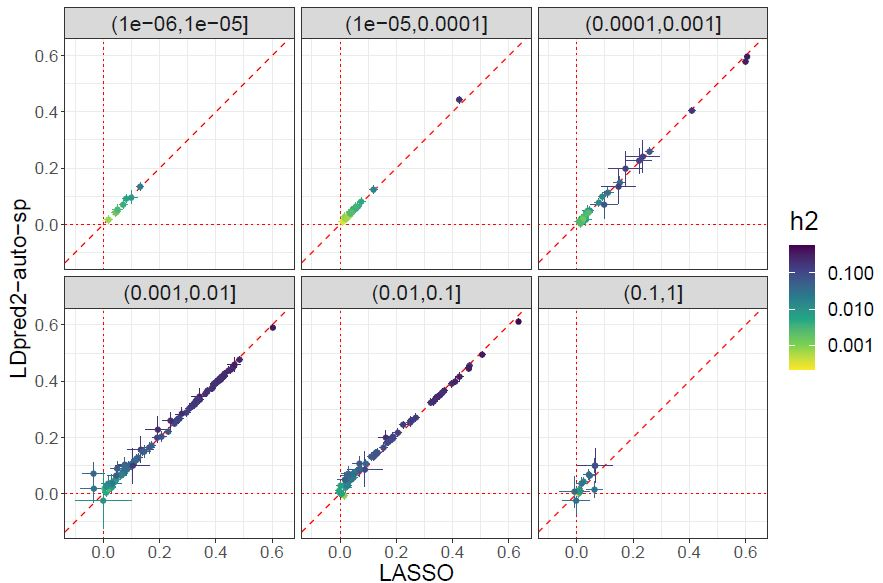
\includegraphics[width=0.9\textwidth]{PLR-ldpred2}
	\caption{}
	\label{fig:plr-ldpred2}
\end{figure}

\begin{figure}[h]
\centering
\includegraphics[width=0.9\textwidth]{sparse-ldpred2}
\caption{}
\label{fig:sparse-ldpred2}
\end{figure}

\begin{figure}[h]
	\centering
	\includegraphics[width=0.8\textwidth]{sparsity-plr}
	\caption{}
	\label{fig:sparsity-plr}
\end{figure}

\begin{figure}[h]
	\centering
	\includegraphics[width=0.8\textwidth]{sparsity-ldpred2}
	\caption{}
	\label{fig:sparsity-ldpred2}
\end{figure}

%%%%%%%%%%%%%%%%%%%%%%%%%%%%%%%%%%%%%%%%%%%%%%%%%%%%%%%%%%%%%%%%%%%%%%%%%%%%%%%%

\begin{figure}[h]
	\centering
	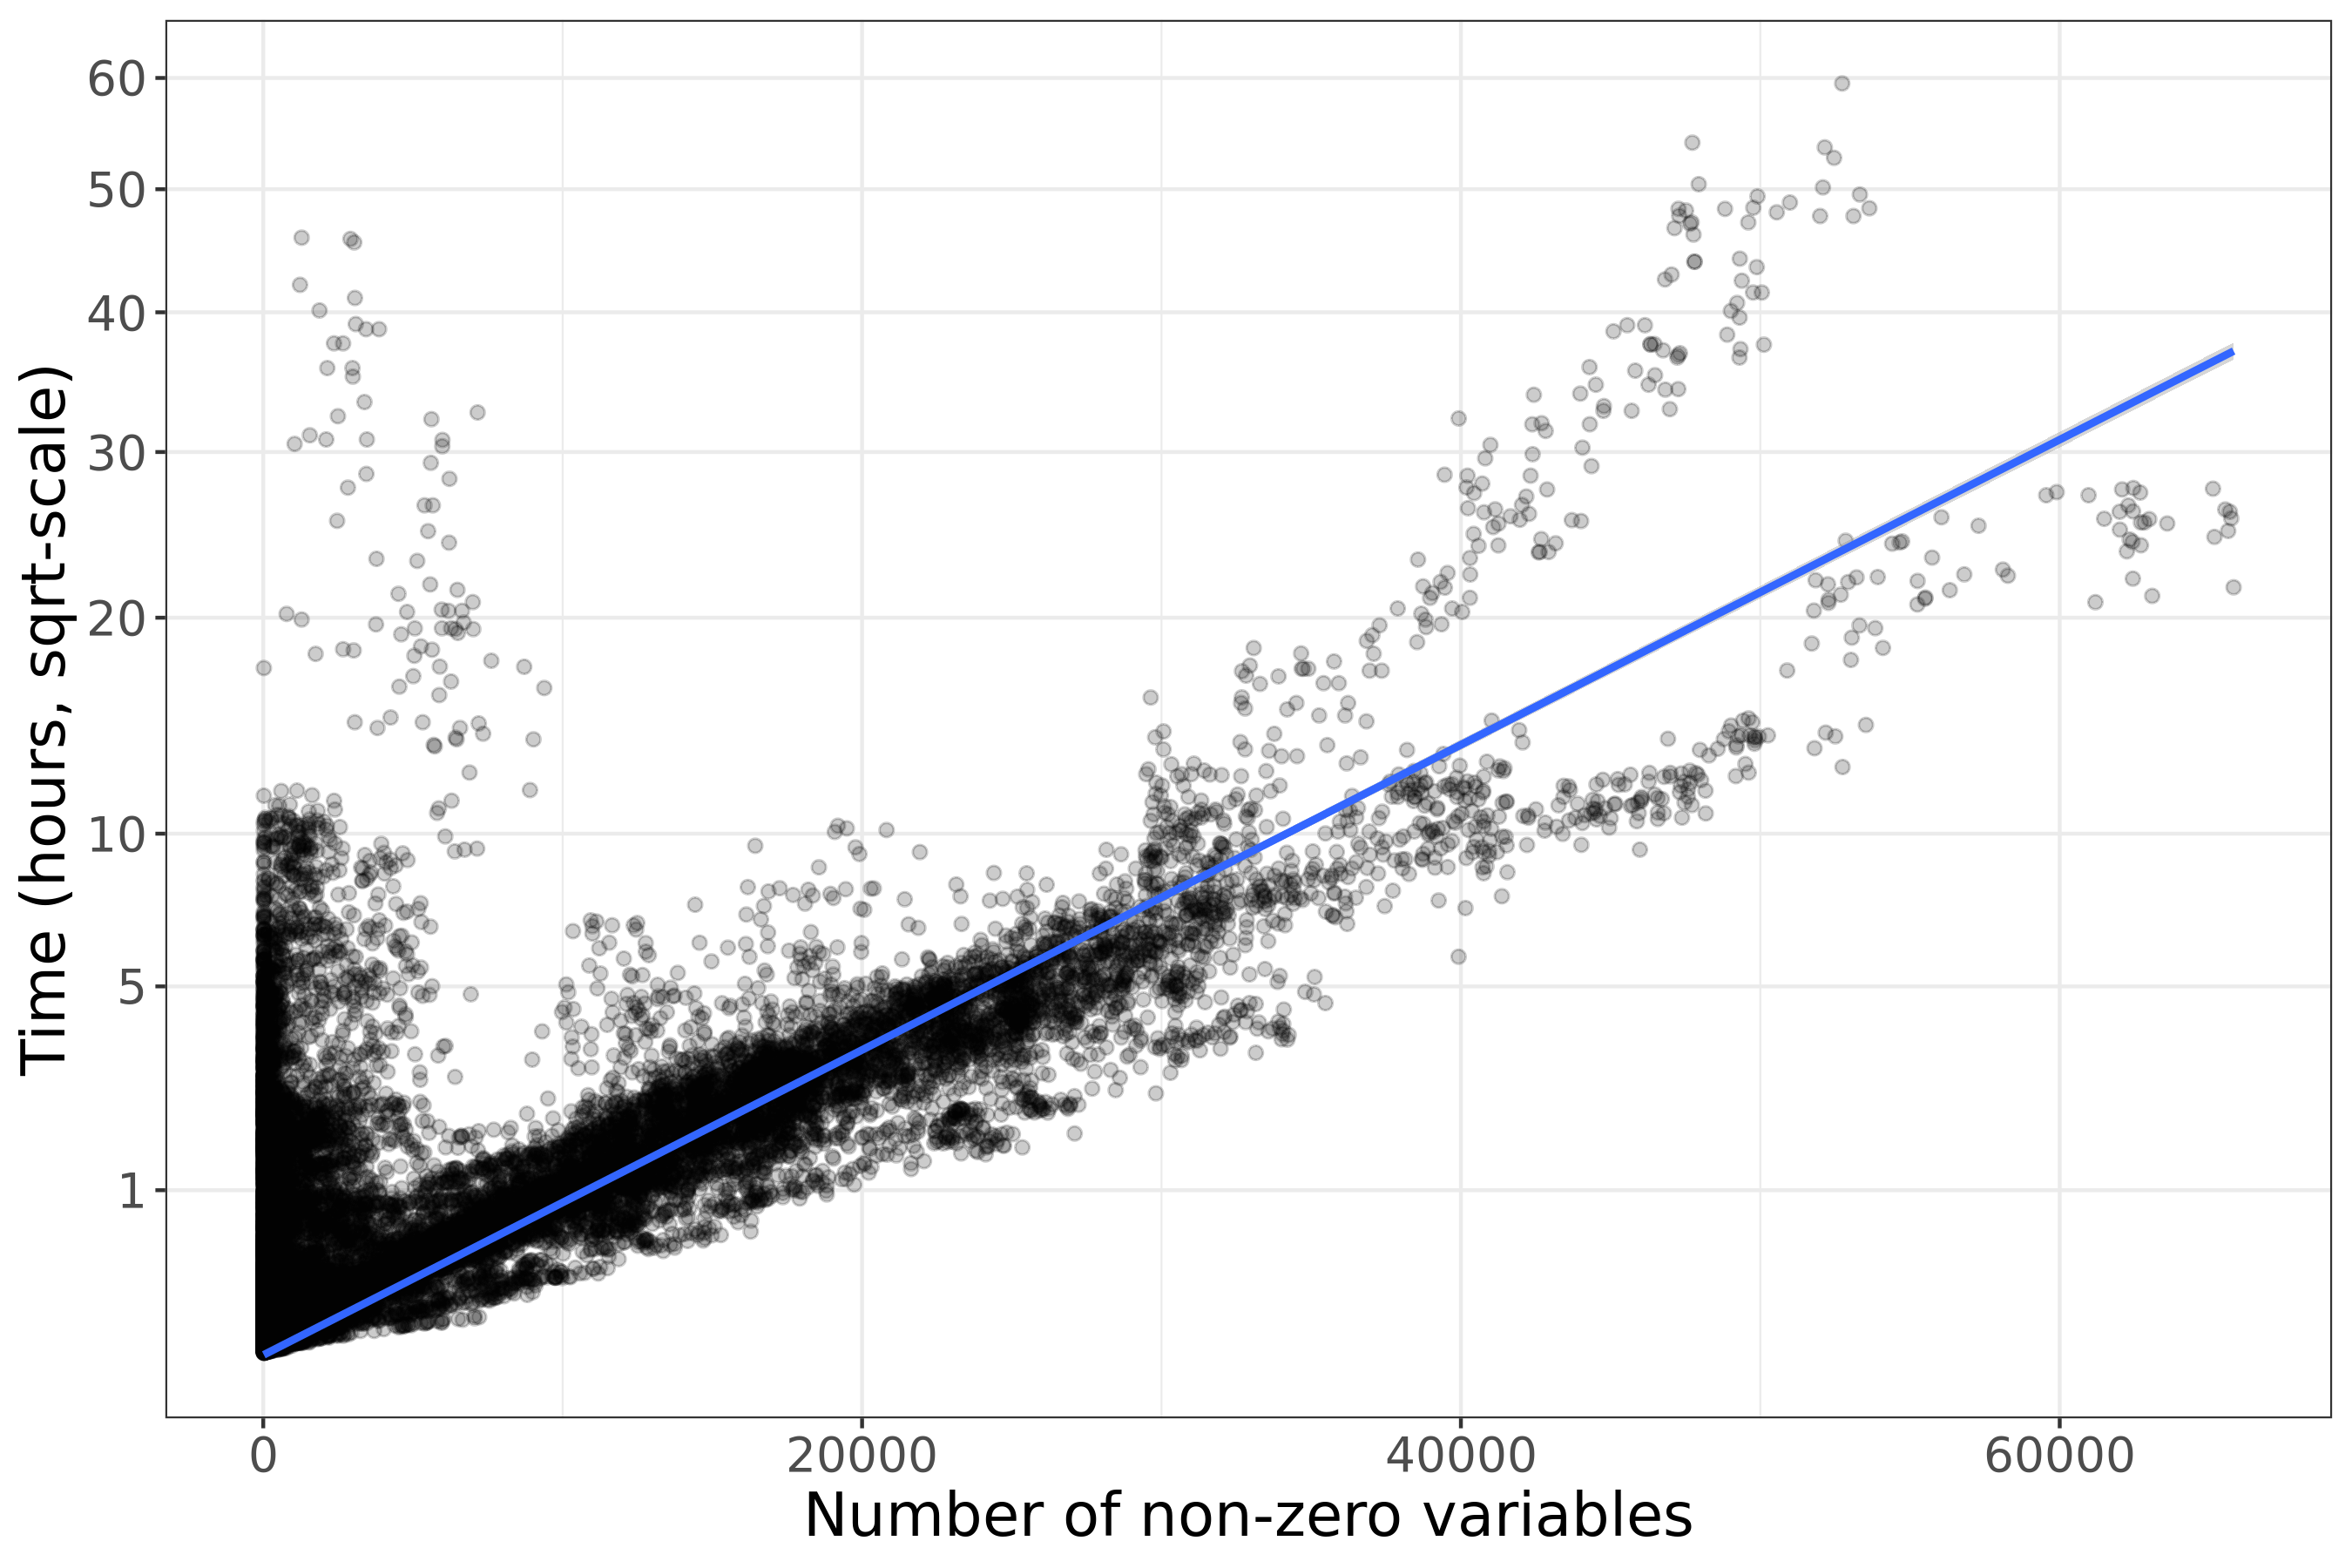
\includegraphics[width=0.9\textwidth]{timings}
	\caption{Computation times for all penalized regression models run using the 1M HapMap3 variants. We recall that we usually run 90 models for each phenotype because we use 9 sets of hyper-parameters and K=10 folds. Computation time is largely quadratic with the number of non-zero effects in the model. It is also dependent on the compute node and the loading of the HPC cluster at the time of running (Figure \ref{fig:timings-ldpred2}).}
	\label{fig:timings-plr}
\end{figure}

\begin{figure}[h]
	\centering
	\includegraphics[width=0.9\textwidth]{timings-ldpred2}
	\caption{Computation times for fitting LDpred2-auto (with default 1000 burn-in iterations + 500 more + sparse option running 150 more) using the 1M HapMap3 variants. Running times should be the same for all phenotypes, yet we see some variability depending on the node used. Some fitting had to be run again because it exceeded the 12-hour timeout, which happened a few times when and the HPC cluster was particularly crowded.}
	\label{fig:timings-ldpred2}
\end{figure}

%%%%%%%%%%%%%%%%%%%%%%%%%%%%%%%%%%%%%%%%%%%%%%%%%%%%%%%%%%%%%%%%%%%%%%%%%%%%%%%%

\begin{figure}[h]
	\centering
	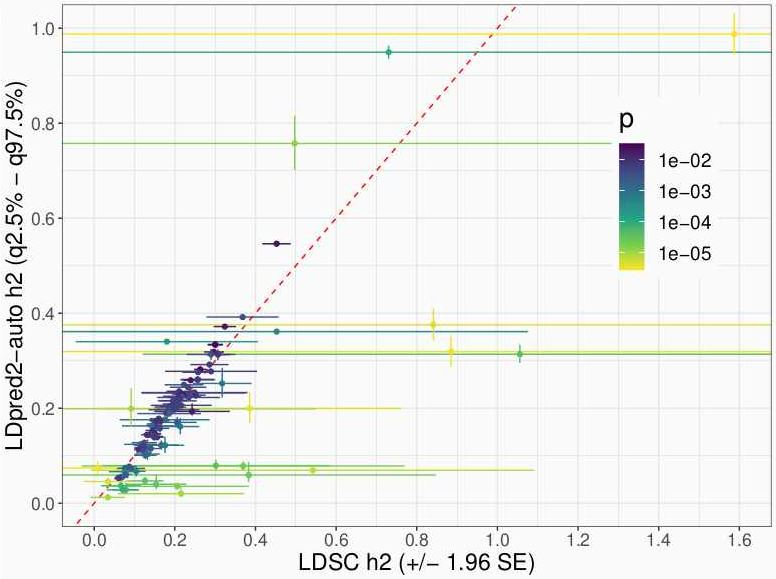
\includegraphics[width=0.9\textwidth]{heritability}
	\caption{}
	\label{fig:heritability}
\end{figure}

\begin{figure}[h]
\centering
\includegraphics[width=0.9\textwidth]{ldpred2-heritability-quant}
\caption{}
\label{fig:heritability-quant}
\end{figure}

\begin{figure}[h]
\centering
\includegraphics[width=0.9\textwidth]{ldpred2-heritability-binary}
\caption{}
\label{fig:heritability-binary}
\end{figure}

\begin{figure}[h]
	\centering
	\includegraphics[width=0.8\textwidth]{sparsity-plr}
	\caption{}
	\label{fig:sparsity-plr}
\end{figure}

%%%%%%%%%%%%%%%%%%%%%%%%%%%%%%%%%%%%%%%%%%%%%%%%%%%%%%%%%%%%%%%%%%%%%%%%%%%%%%%%

\begin{figure}[htbp]
	\centerline{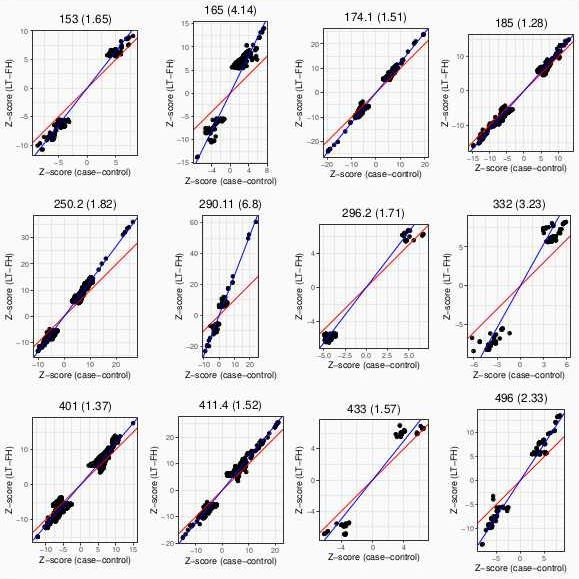
\includegraphics[width=0.95\textwidth]{power_LTFH}}
	\caption{Z-Scores from GWAS using case-control phenotypes and LT-FH phenotypes. Only genome-wide significant variants are represented. The slope (in blue) is computed using Deming regression using the inverse of the absolute value as standard deviations (to put more weight on the more significant variants).
	In the title are reported the phecode as well as this slope (squared), which we report as the power multiplier.}
	\label{fig:power-ltfh}
\end{figure}

\begin{figure}[htbp]
\begin{subfigure}{\textwidth}
\centering
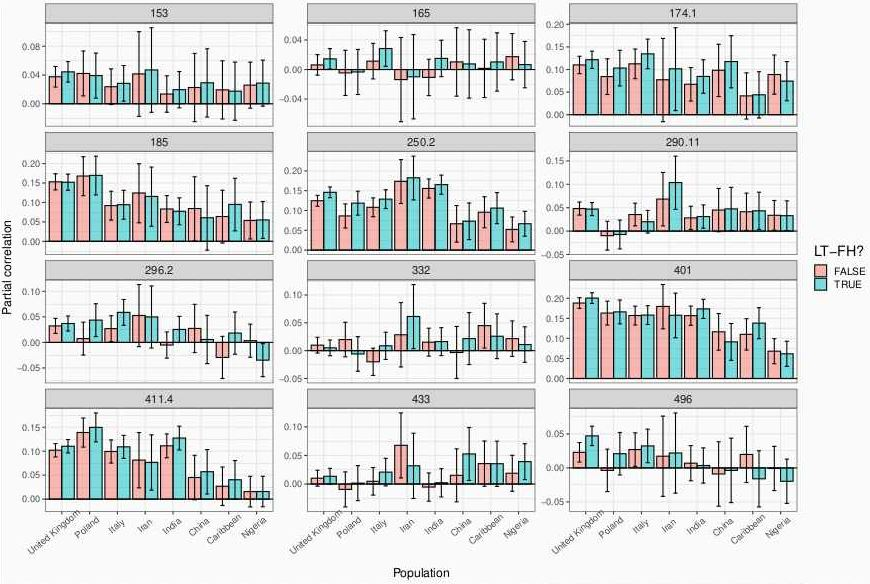
\includegraphics[width=.85\linewidth]{lasso_LTFH}
\end{subfigure}\vspace{1em}
\begin{subfigure}{\textwidth}
\centering
\includegraphics[width=.85\linewidth]{lasso_LTFH2}
\end{subfigure}
\caption{Two subfigures presenting the same results, the partial correlation achieved per phenotype and per population when using either the normal case-control phenotype for training or the phenotype derived using LT-FH. Partial correlations are always derived using the case-control phenotypes in the test set.}
\label{fig:lasso-ltfh}
\end{figure}

%%%%%%%%%%%%%%%%%%%%%%%%%%%%%%%%%%%%%%%%%%%%%%%%%%%%%%%%%%%%%%%%%%%%%%%%%%%%%%%%

\begin{figure}[htbp]
	\centerline{\includegraphics[width=0.9\textwidth]{qc-plot-new-formula}}
	\caption{Comparison of the standard deviations (SD) computed from both genotypes and summary statistics for the 1000 most associated variants with bilirubin concentration. A) uses the previous formula $\text{sd}(\boldsymbol{G_j}) \approx \frac{\text{sd}(\boldsymbol{y})}{\sqrt{n ~ \text{se}(\hat{\gamma}_j)^2}}$ proposed in \cite{prive2020ldpred2} while B) uses the updated formula $\text{sd}(\boldsymbol{G_j}) \approx \frac{\text{sd}(\boldsymbol{y})}{\sqrt{n ~ \text{se}(\hat{\gamma}_j)^2 + \hat{\gamma}_j^2}}$ proposed here, which does one less approximation.
	The slope slightly larger than 1 can be explained by $\text{sd}(\boldsymbol{y}) > \text{sd}(\boldsymbol{\breve{y}})$.}
	\label{fig:new-formula}
\end{figure}

%%%%%%%%%%%%%%%%%%%%%%%%%%%%%%%%%%%%%%%%%%%%%%%%%%%%%%%%%%%%%%%%%%%%%%%%%%%%%%%%

\clearpage


%%%%%%%%%%%%%%%%%%%%%%%%%%%%%%%%%%%%%%%%%%%%%%%%%%%%%%%%%%%%%%%%%%%%%%%%%%%%%%%%

\clearpage

\bibliographystyle{natbib}
\bibliography{refs}

\end{document}
